\documentclass[10pt,a4paper]{article}
\usepackage[margin=2.2cm]{geometry}
\usepackage{fontspec}
\usepackage{kotex}
\setmainfont{Apple SD Gothic Neo}
\setsansfont{Apple SD Gothic Neo}
\usepackage{amsmath,amssymb}
\usepackage{graphicx}
\usepackage{caption}
\usepackage[dvipsnames]{xcolor}
\usepackage[colorlinks=true,linkcolor=MidnightBlue,citecolor=MidnightBlue,
            urlcolor=MidnightBlue]{hyperref}
\usepackage{titlesec}
\titleformat{\section}{\large\bfseries}{\thesection}{0.6em}{}
\captionsetup{font=small,labelfont=bf}
\setlength{\parskip}{0.35em}
\setlength{\parindent}{0pt}
\usepackage{mdframed}
\newmdenv[linewidth=0.4pt,linecolor=gray!60,backgroundcolor=gray!5,
          innertopmargin=6pt,innerbottommargin=6pt,skipabove=8pt,skipbelow=8pt]{claimbox}
\newcommand{\claim}[2]{\begin{claimbox}\textbf{주장.} #1\par\smallskip
  \textcolor{gray!70}{\textbf{반증 조건.} #2}\end{claimbox}}

\title{\bfseries 붕괴선은 결측선이었다\\[2pt]
\large 라벨이 오기 전에 자를 다듬는 리허설 --- 그리고 봉인의 지문 사슬을 복원했다}
\author{월드모델 실험실 · 노트 $845$}
\date{2026-08-08}
\begin{document}\maketitle

\section{한 줄}

첫 전향 봉인($844$ · 개봉 전 $30$편)의 수확 자를 티처 \#$11$ 이 다섯 군데서
찔렀고, 첫 라벨 관측($8/12$) \textbf{전}의 마지막 청정 창에서 리허설로 전부
쟀다. 가장 큰 것: 봉인 풀의 결측(배급 $43.3\%$ · 등급 $16.7\%$)을 판-내 유보
$406$행에 씌우기만 해도 기준 $\rho$ 가 $0.4858 \to \mathbf{0.2101 \pm 0.045}$
로 무너진다 --- \textbf{동결 문턱 $0.2046$('붕괴선')과 사실상 겹친다.} 문턱
미달의 정체는 드리프트가 아니라 결측일 공산이 크다.

\begin{figure}[t]\centering
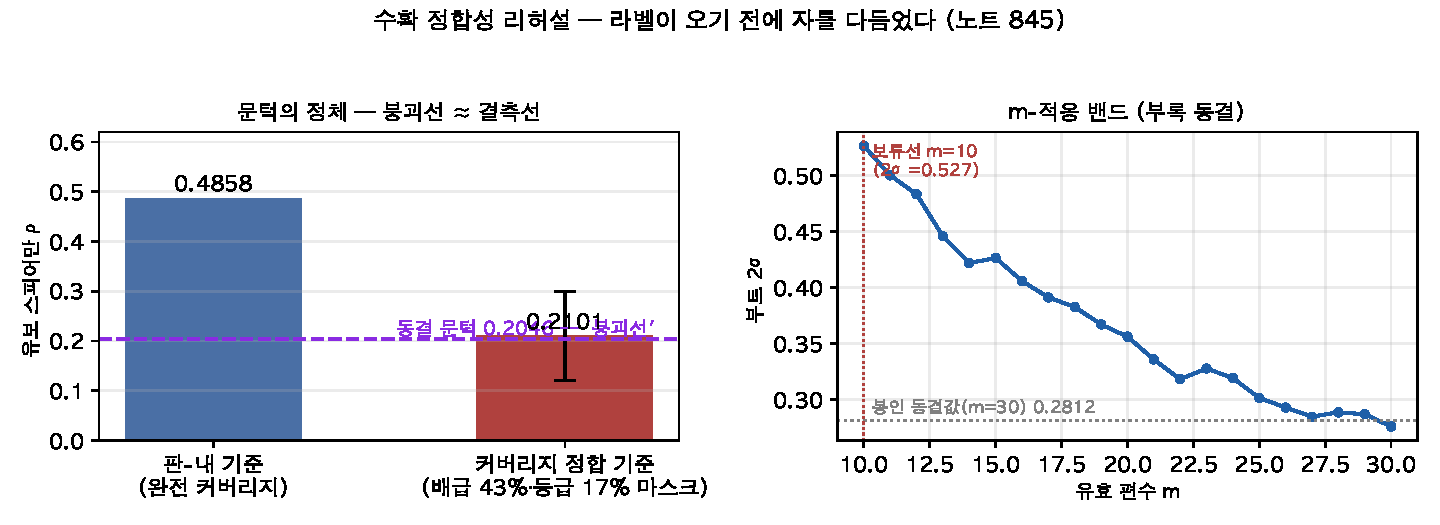
\includegraphics[width=0.97\textwidth]{figs/maskline.pdf}
\caption{왼쪽: 커버리지 정합 기준($6$뽑기 $\pm2$SD)이 동결 문턱과 겹친다.
오른쪽: $m$-적응 밴드(부록 동결) --- 검열로 유효 편수가 줄면 밴드가 급히
넓어진다.}
\end{figure}

\claim{\textbf{수확 판정의 해석 층을 부록으로 분리했다(동결 문면은 불가침).}
통과($\rho \ge 0.2046$)는 ``전향 재현''이 아니라 \emph{``총붕괴 아님''}까지만
--- 죽은 모형($\rho=0$, $n=30$)도 $13.6\%$ 확률로 넘는 문턱이다. 미달은
``붕괴''가 아니라 \emph{``결측 조정 후 재판정''} --- 정합 기준 $0.2101$ 대비로
읽는다. `전향 재현' 상표는 합산 규칙(월별 봉인 가중결합 · 부록 동결)에서
누적 유효 $\ge 60$편부터만 쓴다. 검열은 무해했다(률 $4.7\%$ · 순위 상관
$p=0.091$ 비유의 · 채점 이동 $0.013$).}
{내 효과 크기 예측이 또, 크게 틀렸다: 커버리지 하락 $0.01\sim0.05$ 에 $60\%$
를 걸었는데 실측 $0.276$ --- $5\sim28$배 미스. 이 미스의 정보가 본론보다
클 수 있다: \textbf{영화 도메인 신호의 대부분이 배급 사전 축 하나에 실려
있다}($837$ 의 ``축 $3$개로 판 평균급''은 사실상 ``축 $1$개$+\alpha$'').
개봉 전 배급 확보율이 곧 전향 성능의 지렛대다. `배선 예측은 맞고(지문 복원
적중) 크기 예측은 틀린다' 무늬 $3$연속.}

\section{정직}

정합 기준의 마스크는 무작위인데 봉인의 결측은 소형(사전 밖 배급) 편향이라
근사다($6$뽑기 SD $0.045$). 봉인 후 러너 편집이 지문 사슬을 끊었던 것(티처
\#$11$ 적발 ①)은 편집 역산 재구성이 봉인 sha 와 \textbf{정확 일치}해
복원됐다(\texttt{runners/seal844\_sealed.py} + 사이드카 $2$호 자백). GitHub
흐름 $7$회째(이슈 \#$16 \to$ PR \#$17$). 판 $\rho$ $0.4710$ 그대로.

\end{document}
